\documentclass[11pt,a4paper]{article}
\usepackage{fontspec}
\usepackage[spanish,es-noshorthands]{babel}
\usepackage{amsmath,amssymb,mathtools}
\usepackage[a4paper,margin=2.5cm]{geometry}
\usepackage{booktabs,array}
\usepackage[dvipsnames]{xcolor}
\usepackage{graphicx}
\usepackage{enumitem}
\usepackage{microtype}
\usepackage[font=small,labelfont=bf,labelsep=period]{caption}
\usepackage{titlesec}
\usepackage[colorlinks=true,linkcolor=NavyBlue,citecolor=NavyBlue,urlcolor=NavyBlue]{hyperref}
\numberwithin{equation}{section}
\setlength{\parindent}{1.2em}\setlength{\parskip}{0.2em}
\titleformat{\section}{\large\bfseries\color{NavyBlue}}{\thesection}{0.6em}{}
\titleformat{\subsection}{\normalsize\bfseries}{\thesubsection}{0.5em}{}
\graphicspath{{../codigo/figuras/}{codigo/figuras/}}
\newcommand{\MP}{M_{\rm P}}\newcommand{\kap}{\kappa}\newcommand{\Lb}{\bar\lambda}\newcommand{\dd}{\mathrm d}\newcommand{\ee}{\mathrm e}
\newcommand{\etq}[1]{\,{\footnotesize\color{gray}[#1]}}

\title{\textbf{Espectro tensorial primordial en gravedad unimodular con difusi\'on:\\ ecuaci\'on de los modos y comparaci\'on con RG}}
\author{Javier Pineau\\ \small Curso GW IA --- Entrega final}
\date{28 de septiembre de 2026}

\begin{document}
\maketitle
\begin{abstract}
\noindent
Se estudia si la difusión de energía-momento en gravedad unimodular (UG) modifica el espectro tensorial primordial respecto de la relatividad general (RG). Para materia sin tensión anisótropa TT, la ecuación lineal de los modos sobre un fondo FLRW plano coincide con la de RG (verificado simbólicamente a primer orden): la difusión entra solo a través del fondo. La amplitud cuántica se calcula adoptando la acción tensorial estándar como hipótesis efectiva. Con un inflatón y una difusión prescripta $Q(N)$, el signo de la diferencia depende del criterio de comparación: con el potencial cuadrático, UG suprime la potencia a igual número de onda comóvil y la aumenta en un factor $1.5$--$1.6$ a igual número de e-folds antes del final; con Starobinsky, la diferencia es de $\approx10\%$ a igual número de e-folds y de $5$--$20\%$ a igual número de onda. Para un escalar canónico, una ley local $Q(\phi)$ reduce UG a RG con un potencial efectivo, de modo que esas comparaciones contrastan, en rigor, dos potenciales. Con los fondos de radiación con difusión de \cite{leon22,piccirilli23}, un inflatón de RG reconstruido con el mismo $H(N)$ reproduce el espectro tensorial. El sector escalar no se deriva: las amplitudes escalares de la literatura se comparan de forma condicional. El código, las pruebas y el registro de procedencia acompañan al trabajo en un repositorio reproducible.
\end{abstract}

\section{Introducci\'on}
En gravedad unimodular (UG) el elemento de volumen se fija con un multiplicador de Lagrange, la constante cosmol\'ogica aparece como constante de integraci\'on y las ecuaciones de campo son las de Einstein sin traza \cite{bengochea23}. La conservaci\'on de $T^{ab}$ no es una consecuencia de la teor\'ia sino una hip\'otesis adicional; si se la relaja \cite{josset17}, $\nabla_aT^{ab}=\nabla^bQ$ con $Q$ una funci\'on escalar (la \emph{difusi\'on}) y el multiplicador queda $\lambda=\Lambda_0+\kap Q$. La literatura ha usado esa libertad para estudiar inflaci\'on sin inflat\'on, con radiaci\'on y $Q$ homog\'eneo, y calcular el espectro escalar \cite{leon22,piccirilli23}. La literatura sobre ondas gravitacionales en UG no conservativa es escasa \cite{fabris22}. La pregunta de este trabajo es: \emph{¿cambia $P_T(k)$ respecto de RG cuando $Q$ var\'ia?} El trabajo tiene cuatro partes: (i) derivaci\'on del sector tensorial y su verificaci\'on simb\'olica (secci\'on~\ref{sec:tensores}); (ii) un c\'alculo num\'erico con un inflat\'on y dos potenciales, con dos criterios de comparaci\'on (secci\'on~\ref{sec:inflaton}); (iii) un an\'alisis de consistencia del acoplamiento de $Q$ a la materia (secci\'on~\ref{sec:acopl}); y (iv) el c\'alculo con el fondo descrito en el art\'iculo de 2022 \cite{leon22} (secci\'on~\ref{sec:leon}). Lo que \emph{no} se hace: el sector escalar de UG con difusi\'on (donde hay una discrepancia de un factor $3^{3/2}$ entre \cite{leon22} y \cite{piccirilli23}) ni el recalentamiento.

\paragraph{Convenciones.} $\MP=1/\sqrt{\kap}$ (masa de Planck reducida), $c=\hbar=1$. Las f\'ormulas del texto son dimensionales (con $\MP$ expl\'icita) salvo las de las secciones~\ref{sec:inflaton}--\ref{sec:leon} que se declaran en unidades $\MP=1$ (el código usa $\MP=1$; para los modelos con inflatón integra además con la escala del potencial igual a uno y restaura su valor físico al calcular $P_T$). Cada resultado lleva su procedencia: \etq{P} propio, \etq{C} citado, \etq{E} est\'andar, \etq{S} supuesto o decisi\'on de modelado.

\section{UG con difusi\'on y el fondo cosmol\'ogico}
\label{sec:fondo}
Con el multiplicador $\lambda$ las ecuaciones de campo son $G_{ab}+\lambda g_{ab}=\kap T_{ab}$, la traza fija $\lambda=(R+\kap T)/4$ y la identidad de Bianchi da
\begin{equation}
\nabla_aT^{ab}=\nabla^bQ,\qquad \lambda=\Lambda_0+\kap Q(x),
\label{eq:Qdef}
\end{equation}
con $\Lambda_0$ constante de integraci\'on \etq{C}. En FLRW plano, con $\rho,p$ totales,
\begin{equation}
3\MP^2H^2=\rho+Q+\Lambda_0\MP^2,\qquad -2\MP^2\dot H=\rho+p,\qquad \dot\rho+3H(\rho+p)=-\dot Q.
\label{eq:friedmann}
\end{equation}
$Q$ suma como un fluido con $w=-1$ de densidad variable, y $\Lambda_0=3H_{\rm ini}^2-(\rho_{\rm ini}+Q_{\rm ini})/\MP^2$ \etq{P} (dimensi\'on de masa$^2$; con las mismas condiciones iniciales en RG y UG, $\Lambda_0=-Q_i/\MP^2$). Para el modelo con inflat\'on, la ecuaci\'on que hace consistentes \eqref{eq:friedmann} es $\ddot\phi+3H\dot\phi+V'=-\dot Q/\dot\phi$ \etq{S}; en RG $Q\equiv0$ y $\Lambda_0=\Lambda$.

\section{El sector tensorial}
\label{sec:tensores}
Con $g_{ij}=a^2(\delta_{ij}+h_{ij})$, $\partial_ih_{ij}=h_{ii}=0$, y $\lambda$ escalar (pura traza), la parte TT de $G^i{}_j+\lambda\delta^i_j=\kap T^i{}_j$ es $\delta G^i{}_j|_{\rm TT}=\kap\,\delta T^i{}_j|_{\rm TT}=0$ para un inflat\'on o un fluido perfecto. Se verific\'o con SymPy que para $g=\mathrm{diag}(-1,a^2(1+\varepsilon h),a^2(1-\varepsilon h),a^2)$, $h=h(t,z)$,
\begin{equation}
G^x{}_x-G^y{}_y=\varepsilon\Big(\ddot h+3H\dot h-\frac{\partial_z^2h}{a^2}\Big)+O(\varepsilon^2),
\label{eq:GxxGyy}
\end{equation}
de modo que
\begin{equation}
\boxed{\ \ddot h_k+3H\dot h_k+\frac{k^2}{a^2}h_k=0\ }
\label{eq:modok}
\end{equation}
\emph{es la ecuaci\'on de RG}; $Q$ y $\Lambda_0$ entran solo por $H(t)$ \etq{P, verificada a primer orden}. En tiempo c\'osmico el v\'inculo es $\sqrt{-g}=f(t)=a^3(t)$; con la parametrizaci\'on lineal $g_{ij}=a^2(\delta_{ij}+h_{ij})$, a segundo orden $\sqrt{-g}-f=-\tfrac14 a^3h_{ij}^2+O(h^3)$ (la parametrizaci\'on $g_{ij}=a^2(\ee^h)_{ij}$ lo cumple a todo orden). Para calcular la amplitud cuántica se adopta, adicionalmente, la acción tensorial estándar como hipótesis de la realización efectiva. La expansión manual que la motiva usa la contribución de materia $S_m^{(2)}\supset-a^3p\,h_{ij}^2/4$. Bajo esa elección, el término del multiplicador, $+\bar\lambda a^3h_{ij}^2/(4\kap)$, participa en la cancelación del término de masa por la ecuación de fondo. El término gradiente se toma del resultado estándar y se comprueba por consistencia con \eqref{eq:modok}; no se deriva independientemente en este trabajo. Con ese alcance, se utiliza
\begin{equation}
S^{(2)}=\frac{\MP^2}{8}\int\dd t\,\dd^3x\,\big[a^3\dot h_{ij}^2-a(\partial_kh_{ij})^2\big],
\label{eq:S2}
\end{equation}
idéntica a la de RG \etq{S; cancelación de masa P, a mano}. \emph{Alcance.} La ecuaci\'on \eqref{eq:modok} no fija por s\'i sola la normalizaci\'on cu\'antica (multiplicar la acci\'on por una constante no la cambia). La normalizaci\'on de $P_T$ usa \eqref{eq:S2} como \emph{hip\'otesis de la realizaci\'on efectiva}: no se especifica una acci\'on completa de materia que produzca la difusi\'on, y la ``ausencia de tensi\'on anis\'otropa a primer orden'' no equivale a haber justificado la acci\'on de materia a segundo orden (en particular con intercambio de energ\'ia). Un $Q$ variable no sale de una acci\'on covariante est\'andar: es un supuesto compartido con la literatura \cite{fabris22}. Con $e^\lambda_{ij}e^{\lambda'}_{ij}=2\delta^{\lambda\lambda'}$, $v=a\MP h/\sqrt2$, Bunch--Davies y $P_T\equiv\langle h_{ij}h_{ij}\rangle$ por $\ln k$, $P_T=4k^3|v|^2/(\pi^2a^2\MP^2)$ (con $\MP=1$ en el c\'odigo), que en de Sitter da $2H^2/(\pi^2\MP^2)$ \etq{E} \cite{baumann22}.

\section{Inflat\'on con $Q(N)$: dos potenciales y dos criterios}
\label{sec:inflaton}
\paragraph{M\'etodo.} Se integra \eqref{eq:friedmann} con la ecuaci\'on del inflat\'on de la secci\'on~\ref{sec:fondo} (DOP853, $\mathrm{rtol}_{\rm fondo}=10^{-12}$) y, para cada $k$, la ecuaci\'on de $v$ en $N=\ln a$,
$w_{,N}+(1-\epsilon_1)w+[(k/aH)^2-(2-\epsilon_1)-2X/H^2]v=0$, donde $w=\dd v/\dd N$. Los modos se integran también con DOP853, con $\mathrm{rtol}_{\rm modos}=10^{-10}$ y $X=-3H^2-2\dot H-p+\bar\lambda$ (el t\'ermino de masa, que se \emph{calcula} y resulta $\lesssim10^{-15}H^2$; es un control de consistencia algebraica, porque $H$, $\dot H$, $p$ y $\bar\lambda$ se construyen con ecuaciones relacionadas: no prueba de forma independiente la teor\'ia a segundo orden), desde $k/aH=100$ hasta $10^{-3}$. Decisiones \etq{S}: mismos $(\phi_i,\dot\phi_i,H_i)$ en RG y UG (lo que fija $\Lambda_0=-Q_i$); $Q(N)=Q_i\ee^{-\gamma N}$ con $Q_i/V_i=0.1$, $\gamma=0.1$; $\phi_i$ ajustado para que UG dure $N_f=100$ e-folds; potencial cuadr\'atico $V=\tfrac12m^2\phi^2$ ($m=6\times10^{-6}\MP$) y de Starobinsky \cite{starobinsky80,defelice10} $V=\tfrac34M^2\MP^2(1-\ee^{-\sqrt{2/3}\phi/\MP})^2$ ($M=1.14\times10^{-5}\MP$, calibrada con $A_s$ en RG a $N_*=60$ mediante la fórmula escalar slow-roll de orden cero). Solo se usa la forma del potencial de Starobinsky; el origen $R^2$ es de RG. La forma de $Q(N)$ es fenomenol\'ogica. Como se muestra en la secci\'on~\ref{sec:acopl}, sobre la trayectoria considerada estas corridas equivalen a RG con el potencial efectivo $V+Q+\Lambda_0\MP^2$: la diferencia UG--RG de esta secci\'on es una diferencia de fondo, no de la propagaci\'on de los modos.

\paragraph{Resultado a igual $k$.} Con el cuadr\'atico y mismas condiciones iniciales, RG dura $161.8$ e-folds y UG $100$; a igual $k$ comóvil UG suprime $P_T$ (fig.~\ref{fig:fig1}): el cociente va de $0.914$ a $0.344$. La diferencia se explica por el fondo: coincide con el cociente de la f\'ormula est\'andar de RG evaluada con el $H$ y $\epsilon_1$ de UG con una desviación relativa máxima de $2.80\times10^{-5}$ en la muestra de modos del cuadrático que satisface el criterio slow-roll del control (véase el apéndice~\ref{app:validacion}), y no es ruido num\'erico (cociente entre la diferencia de modelos y el error num\'erico estimado: $1.3\times10^5$; no es una significancia estad\'istica ni una detectabilidad experimental). Adem\'as, en UG la inflaci\'on termina antes. Con $K=\dot\phi^2/2$ y $U=V+Q+\Lambda_0\MP^2$ es $3\MP^2H^2=K+U$ y $\epsilon_1=3K/(K+U)$, de modo que la inflaci\'on termina ($\epsilon_1=1$) cuando $U=2K$, igual que en RG con $U=V$. En UG, como $Q(N)<Q_i$, el t\'ermino $Q+\Lambda_0\MP^2=Q-Q_i$ es negativo, resta a $U$ y adelanta ese instante.

\begin{figure}[t]\centering
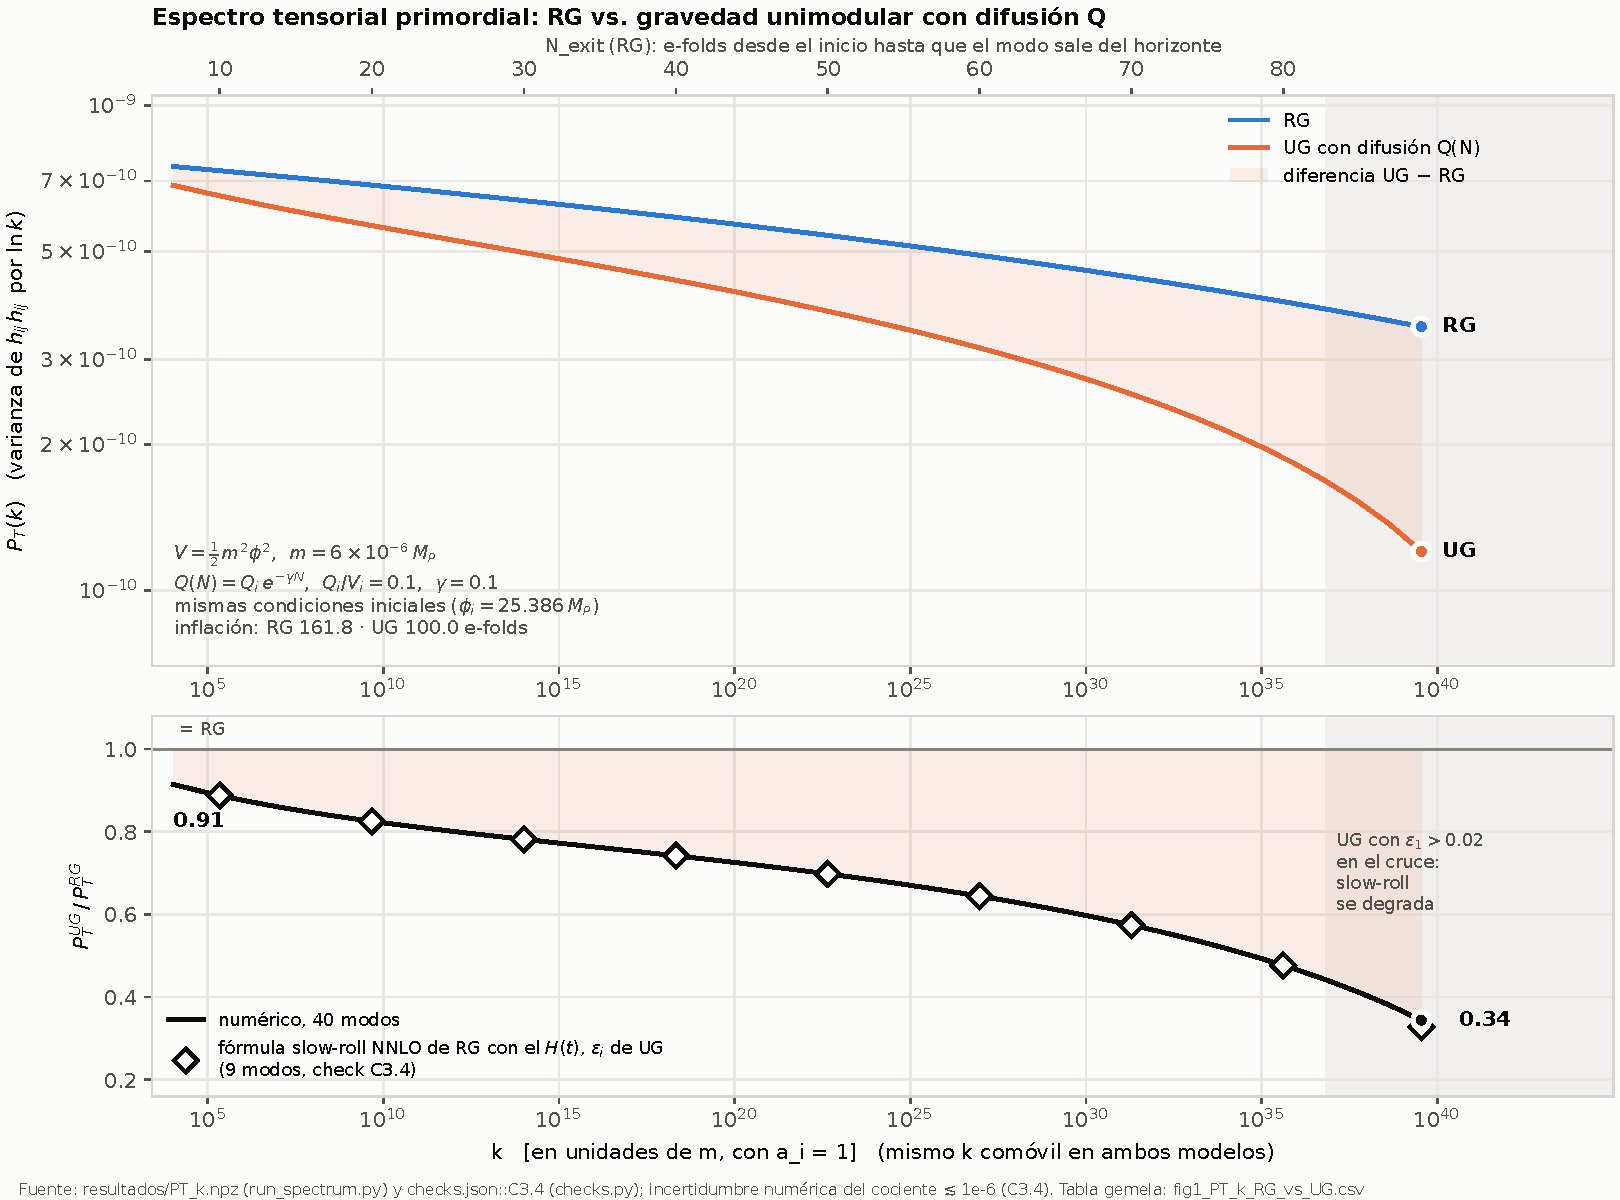
\includegraphics[width=0.92\textwidth]{fig1_PT_k_RG_vs_UG.pdf}
\caption{$P_T(k)$ en RG y UG (cuadr\'atico, mismas condiciones iniciales) y su cociente a igual $k$. Marcadores huecos: slow-roll de RG con el fondo de UG.}
\label{fig:fig1}
\end{figure}

\paragraph{El criterio importa.} A igual $k$ se comparan \'epocas distintas, porque las duraciones difieren (con Starobinsky, $386.7$ frente a $100$; fig.~\ref{fig:fig6}). Una comparaci\'on ilustrativa m\'as cercana a las observaciones es $P_T$ y $n_T$ en el modo que sali\'o $N_*$ e-folds antes del final de \emph{cada} inflaci\'on (es una convenci\'on: identificar el mismo $k_*$ f\'isico exige la historia posterior, el recalentamiento y la normalizaci\'on de $a$, que no se modelan). Con ese criterio (tabla~\ref{tab:igualN}, fig.~\ref{fig:fig8}) \emph{el signo cambia en el cuadr\'atico}: UG aumenta $P_T$ por $1.5$--$1.6$, porque su inflaci\'on termina antes en el potencial ($\phi\approx8.4\,\MP$ contra $\approx1.01\,\MP$ en RG, ambos en $\epsilon_1=1$) y 60 e-folds antes de su final el campo est\'a m\'as arriba y $H$ es mayor. Con Starobinsky la diferencia es menor: el cociente es $0.90$ a igual $N_*$ (una reducci\'on de $\approx10\%$) y va de $0.947$ a $0.796$ a igual $k$ (entre $5$ y $20\%$). All\'i $\Lambda_0=-Q_i$ es el $10\%$ de la altura del plateau y en los pivotes $H_{\rm UG}/H_{\rm RG}\approx0.95$ (de ah\'i $0.95^2\approx0.90$); adem\'as, $|\Delta n_T|<3.1\times10^{-4}$ (no se evalu\'o su detectabilidad); el final de UG cumple $U=2K$; no se aisló el efecto causal de $\Lambda_0$. Adem\'as los primeros $\sim30$ e-folds de UG est\'an dominados por $Q$ ($|Q'|/|V'|\gtrsim1$), consecuencia de imponer las mismas condiciones iniciales.

\begin{figure}[t]\centering
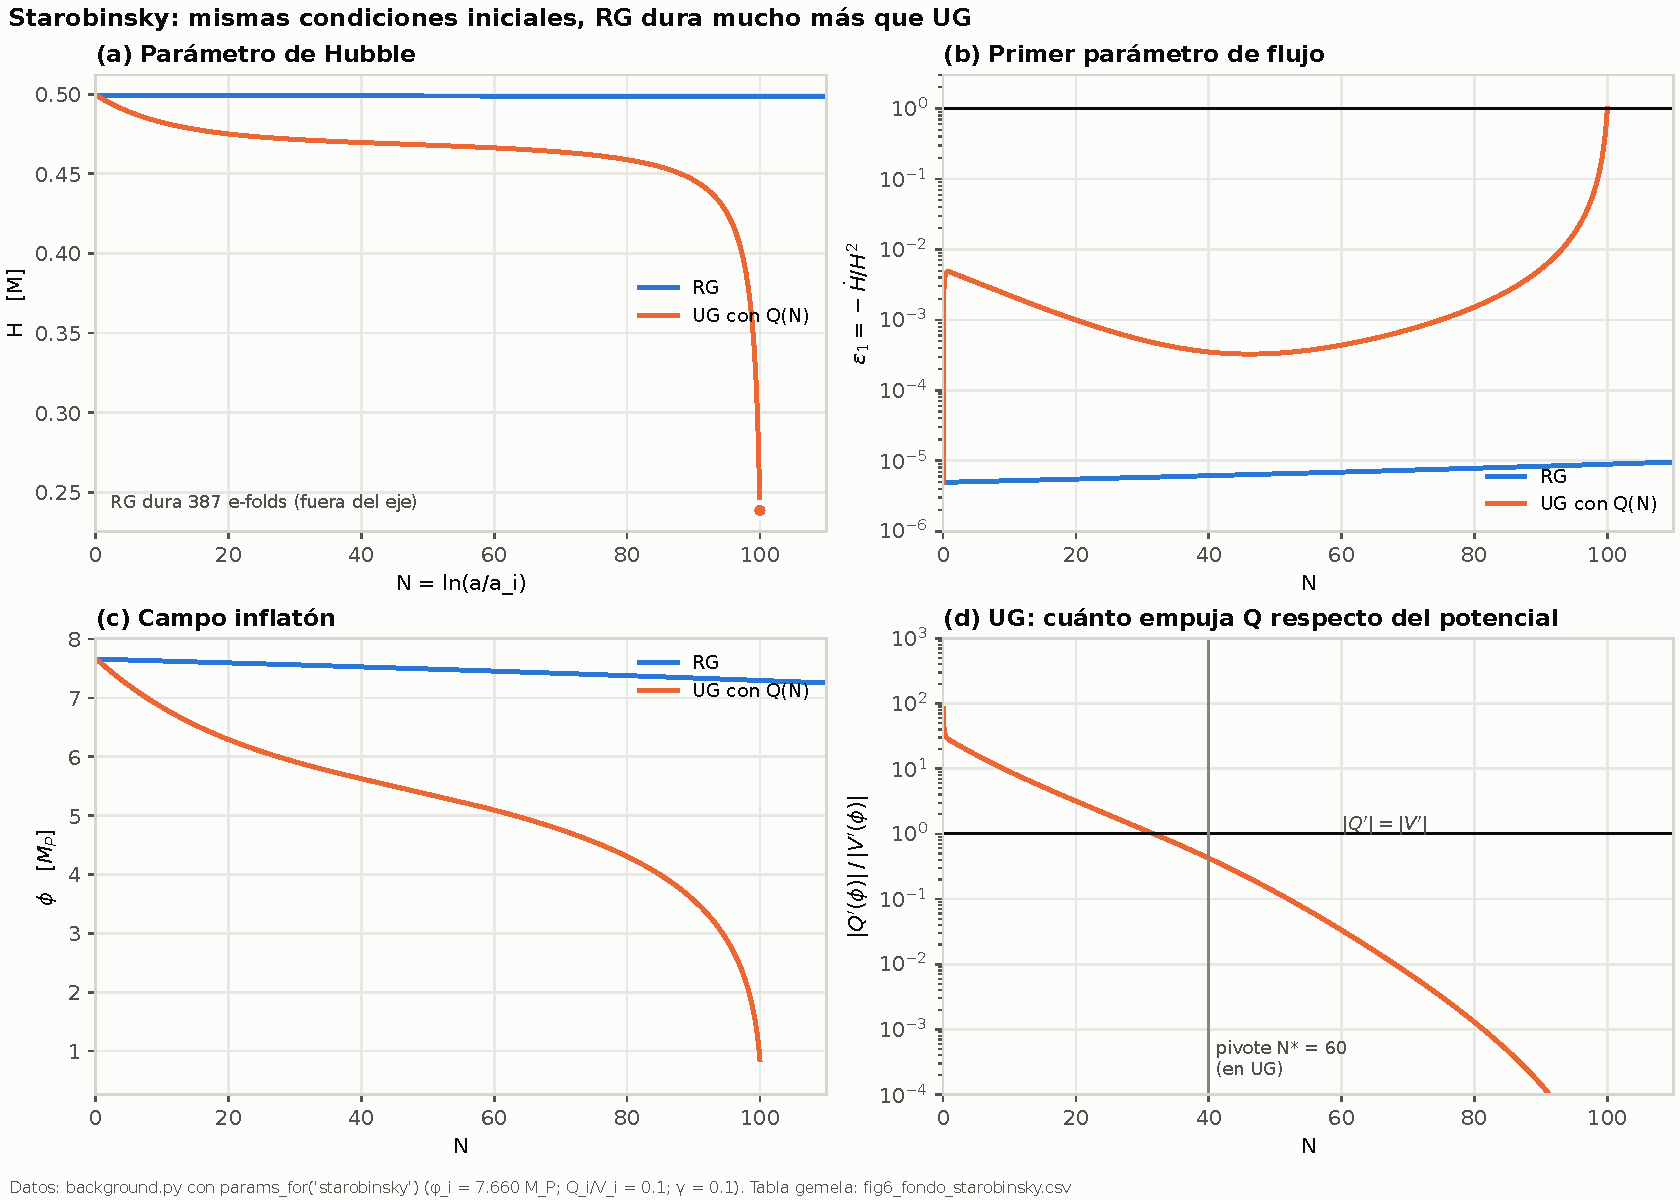
\includegraphics[width=0.92\textwidth]{fig6_fondo_starobinsky.pdf}
\caption{Fondo con el potencial de Starobinsky: (a) $H$, (b) $\epsilon_1$, (c) $\phi$, (d) $|Q'|/|V'|$ en UG.}
\label{fig:fig6}
\end{figure}

\begin{table}[t]\centering\small\renewcommand{\arraystretch}{1.15}
\begin{tabular}{@{}llrrrr@{}}
\toprule
Potencial & $N_*$ & $P_T^{\rm UG}/P_T^{\rm RG}$ & $n_T^{\rm RG}$ & $n_T^{\rm UG}$ & $r_{\rm std}^{\rm RG}\ /\ r_{\rm std}^{\rm UG}$\\
\midrule
cuadr\'atico & 50 & 1.575 & $-2.0\times10^{-2}$ & $-1.6\times10^{-2}$ & 0.160 / 0.125\\
cuadr\'atico & 60 & 1.516 & $-1.7\times10^{-2}$ & $-1.4\times10^{-2}$ & 0.133 / 0.109\\
Starobinsky & 50 & 0.902 & $-5.5\times10^{-4}$ & $-6.7\times10^{-4}$ & $4.4\times10^{-3}$ / $5.4\times10^{-3}$\\
Starobinsky & 60 & 0.904 & $-3.9\times10^{-4}$ & $-7.0\times10^{-4}$ & $3.1\times10^{-3}$ / $5.6\times10^{-3}$\\
\bottomrule
\end{tabular}
\caption{Comparaci\'on a igual $N_*$. $P_T$ y $n_T$ son resultados; $r_{\rm std}=P_T/P_\mathcal{R}^{\rm LO}$ usa la f\'ormula escalar de RG con el fondo de UG (condicional: el sector escalar de UG no est\'a derivado).}
\label{tab:igualN}
\end{table}

\begin{figure}[t]\centering
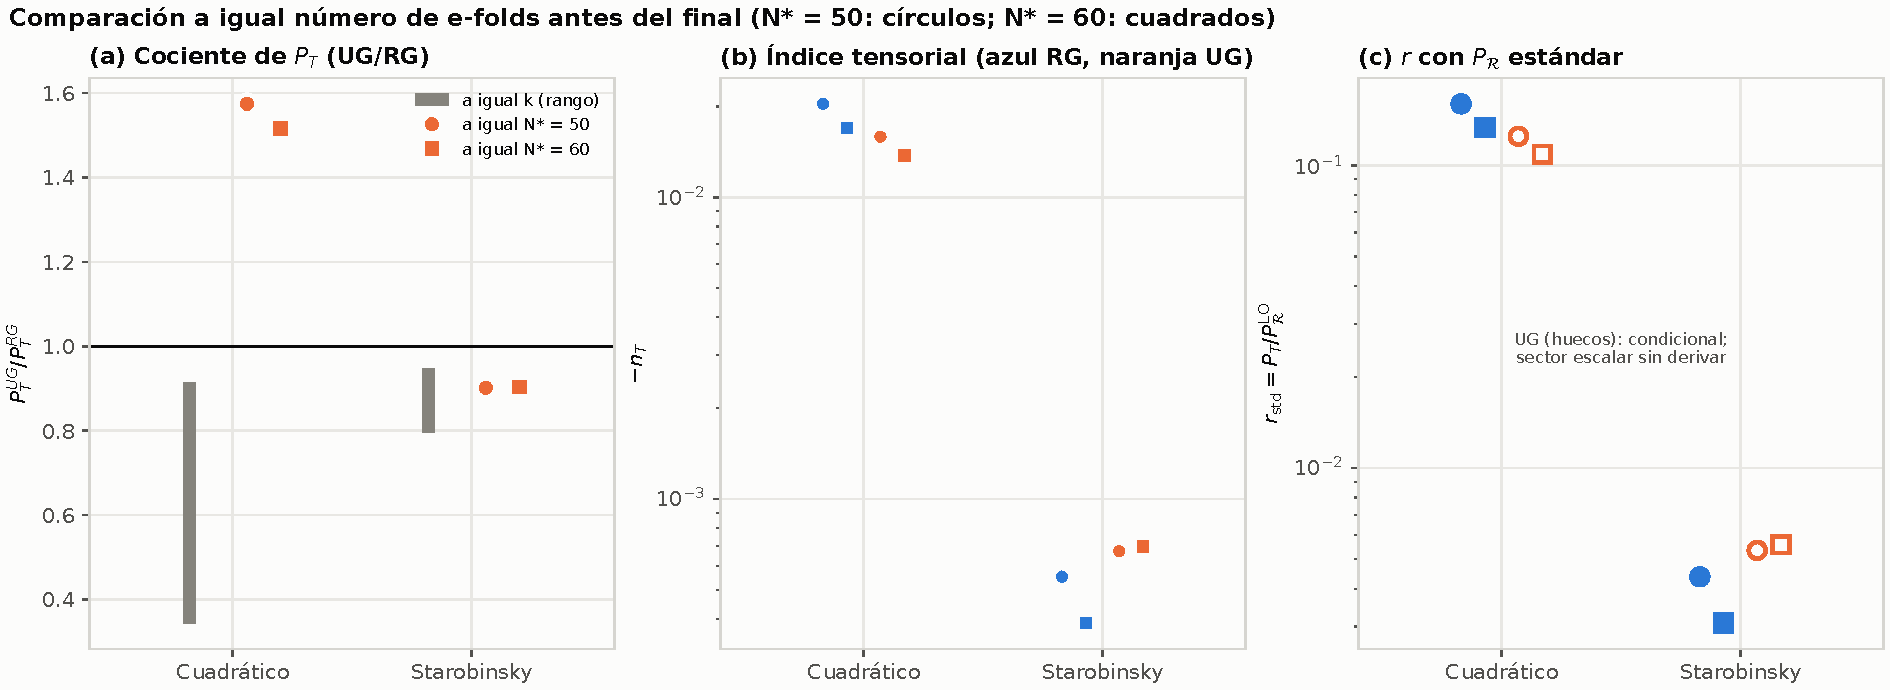
\includegraphics[width=\textwidth]{fig8_igual_Nstar.pdf}
\caption{Igual $N_*$: (a) cociente de $P_T$ (barra gris: rango a igual $k$); (b) $-n_T$; (c) $r_{\rm std}$ (UG condicional).}
\label{fig:fig8}
\end{figure}

\section{¿Es consistente acoplar $Q$ a un inflat\'on?}
\label{sec:acopl}
Para un escalar can\'onico con el tensor energ\'ia-impulso usado, $\nabla_aT^{ab}=(\Box\phi-V')\nabla^b\phi$ (comprobado simb\'olicamente a primer orden con un ansatz escalar sin el modo E y $V$ cuadr\'atico y de Starobinsky). Con \eqref{eq:Qdef}, $\nabla_bQ\parallel\nabla_b\phi$ en \emph{todas} las componentes, luego, donde $\nabla\phi\neq0$ (la conclusi\'on es local; extenderla globalmente requiere hip\'otesis adicionales),
\begin{equation}
Q=Q(\phi),\quad \Box\phi=V'+Q',\quad \delta Q=Q'\delta\phi,\qquad V_{\rm eff}=V+Q(\phi)+\Lambda_0\MP^2 .
\label{eq:Veff}
\end{equation}
\emph{Para un escalar can\'onico y una difusi\'on local especificada como ley $Q(\phi)$, las ecuaciones de UG son las de RG con $V_{\rm eff}$} en el fondo (verificado simb\'olicamente: $\dot H=-\dot\phi^2/2$ y la ecuaci\'on de Klein--Gordon coinciden) y, argumentado a mano, en las perturbaciones. Las corridas de la secci\'on~\ref{sec:inflaton} usan $Q(N)$; su interpretaci\'on como $Q(\phi)=Q(N(\phi))$ requiere reconstruir y fijar esa funci\'on sobre la rama monótona considerada, y no define la misma teor\'ia para otras condiciones iniciales o perturbaciones fuera de la trayectoria. No se afirma una equivalencia irrestricta de teor\'ias, ni de su cuantizaci\'on, a partir de esta cuenta; lo que se afirma es que en esa rama las corridas comparan dos potenciales.

\paragraph{El caso $\delta Q=0$.} La componente espacial da $\partial_x\delta Q=E_0\,\partial_x\delta\phi$ con $E_0=\Box\phi-V'$. Si se impone $\delta Q=0$ \emph{en el marco especificado} y la perturbaci\'on del inflat\'on es inhomog\'enea ($\partial_x\delta\phi\neq0$), entonces $E_0=0$ y $\dot Q=E_0\dot\phi=0$. Dos l\'imites: (i) el producto tambi\'en se anula si $\partial_x\delta\phi=0$ (campo uniforme), rama que el control simb\'olico no descarta ni excluye; (ii) $\delta Q=0$ no es invariante de gauge: para escalares, bajo $t\to t+\xi^0$, $\widetilde{\delta\phi}=\delta\phi-\dot{\bar\phi}\,\xi^0$ y $\widetilde{\delta Q}=\delta Q-\dot{\bar Q}\,\xi^0$ \etq{E}, as\'i que requiere una especificaci\'on de gauge o una condici\'on f\'isica adicional, y su compatibilidad con las transformaciones permitidas y el v\'inculo unimodular no se examin\'o. La extensi\'on a otros gauges o a perturbaciones uniformes exige un an\'alisis adicional, de modo que \emph{no} se afirma que un inflat\'on no pueda intercambiar energ\'ia con $Q$ en general. Esto no invalida el estudio de la radiaci\'on con $Q$ de la secci\'on siguiente como modelo; invalida presentarlo como una necesidad demostrada por este argumento.

\section{El fondo del art\'iculo de 2022: radiaci\'on pura y $Q$ \cite{leon22}}
\label{sec:leon}
Seg\'un el art\'iculo de 2022 \cite{leon22}, con $p=\rho/3$, $\Lambda_0=0$ y $\delta Q=0$, \eqref{eq:friedmann} y $\epsilon_1=2/(1+Q/\rho)$ dan, dada $\epsilon_1(N)$ y una normalizaci\'on \etq{C},
\begin{equation}
H=H_{\rm ref}\ee^{-\int\epsilon_1\dd N},\qquad \rho=\tfrac32\epsilon_1H^2,\qquad Q=\tfrac32(2-\epsilon_1)H^2,
\label{eq:leon}
\end{equation}
y hay inflaci\'on ($\epsilon_1<1$) si $Q>\rho$. Se implementa el escenario 1 de \cite{piccirilli23}, $\epsilon_1=(1+N_f-N)^{-\gamma}$ con $N_f=100$, $\rho_{\rm end}=10^{-11}\MP^4$ y $\gamma=2.02$, y el escenario 3 (mapeo de potenciales slow-roll a $Q(N)$). No se reajusta la escala en esta reproducci\'on: se adopta la normalizaci\'on de la referencia ($\rho_{\rm end}=10^{-11}\MP^4$ es una entrada de la literatura), de modo que la amplitud queda determinada \emph{condicionalmente a esa normalizaci\'on}. El escenario 2 (necesita $N_f\simeq370$) no se analiza.

\paragraph{Resultado tensorial.} $P_T$ depende solo de $H(N)$ y $\epsilon_1(N)$; un inflat\'on de RG con $V=(3-\epsilon_1)H^2$ y $\dd\phi/\dd N=-\sqrt{2\epsilon_1}$ reconstruido da el mismo $H(N)$ (diferencia relativa m\'axima $8\times10^{-7}$) y el mismo $P_T$ (diferencia relativa m\'axima $2\times10^{-8}$ en los 28 modos que alcanzan $q=10^{-3}$ y $\lesssim5\times10^{-11}$ en $N_*=50$ y $60$; los dos modos que salen demasiado cerca del final se muestran aparte en la fig.~\ref{fig:fig10}a). \emph{No hay diferencia UG--RG en el sector tensorial a igual $H(N)$}; est\'a en qu\'e historias $H(N)$ se realizan y en el sector escalar.

\paragraph{Amplitud y $r$ (condicionales).} En el punto de referencia de \cite{piccirilli23} ($\gamma=2.02$, $N_*=57$): $P_T=9.30\times10^{-12}$ y $n_T=-5.5\times10^{-4}$. Con $P_\mathcal{R}=H^2/(8\pi^2\epsilon_1\MP^2)$ (Eq.~41 de \cite{piccirilli23}) resulta $A_s=2.12\times10^{-9}$, $1.1\%$ sobre Planck ($2.099\times10^{-9}$ \cite{planck20}) sin ajustar, y $r=4.4\times10^{-3}$, por debajo de la cota $r<0.036$ de BICEP/Keck \cite{bicep21}; con la de \cite{leon22} (Eq.~66, factor $3^{3/2}$) $A_s=1.10\times10^{-8}$, cinco veces mayor, y con $1/c_s$, $c_s^2=1/3$ (mi hip\'otesis, \emph{no verificada} contra \cite{garriga99}) $3.7\times10^{-9}$ (fig.~\ref{fig:fig10}b). \emph{Esto no dice cu\'al f\'ormula es correcta}: los par\'ametros de \cite{piccirilli23} se eligieron con la suya, y la normalizaci\'on adoptada es la de esa referencia. Para $\gamma=1.5$ ($N_*=60$) $A_s=1.32\times10^{-9}$.

\paragraph{Escenario 3: mapeo de potenciales a radiación con difusión.}
Se toman los parámetros slow-roll de los potenciales cuadrático y de Starobinsky para prescribir $\epsilon_1(N)$ y reconstruir $H$, $\rho$ y $Q$ con \eqref{eq:leon}, usando $\rho_{\rm end}=10^{-11}\MP^4$. Se compara el espectro de ese fondo con el obtenido al integrar el inflatón de RG correspondiente. Esta comparación es distinta de la reconstrucción a igual $H(N)$: el mapeo usa una aproximación slow-roll y no impone la igualdad exacta de los fondos. Para $R=P_T(N_*=60)/P_T(N_*=50)$, la diferencia relativa $|R_{\rm map}/R_{\rm RG}-1|$ es menor que $0.3\%$ en ambos potenciales. Sin embargo, las amplitudes presentan $P_T^{\rm RG}/P_T^{\rm map}-1\simeq23$--$29\%$ en esos puntos. La cercanía de la razón entre dos escalas no demuestra acuerdo de amplitud ni de toda la forma espectral; tampoco se aisló la causa de la discrepancia. El criterio sobre esa razón es exploratorio y se adoptó después del fallo del criterio inicial de amplitud (apéndice~\ref{app:validacion}).

\begin{figure}[t]\centering
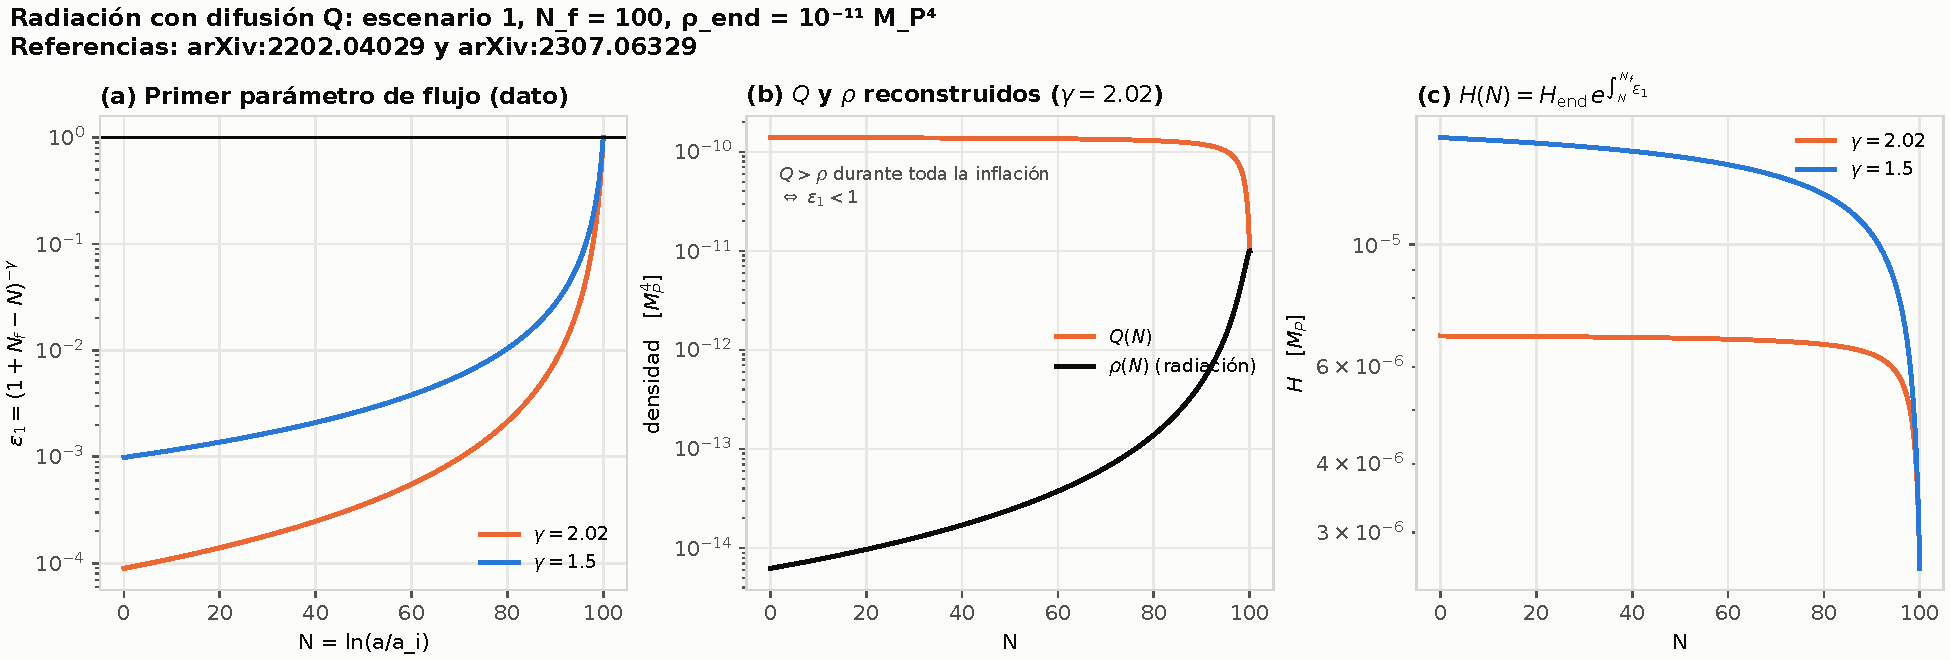
\includegraphics[width=\textwidth]{fig9_fondo_leon.pdf}
\caption{Modelo de radiación con difusión Q \cite{leon22,piccirilli23} (escenario 1): (a) $\epsilon_1(N)$; (b) $Q$ y $\rho$; (c) $H(N)$.}
\label{fig:fig9}
\end{figure}
\begin{figure}[t]\centering
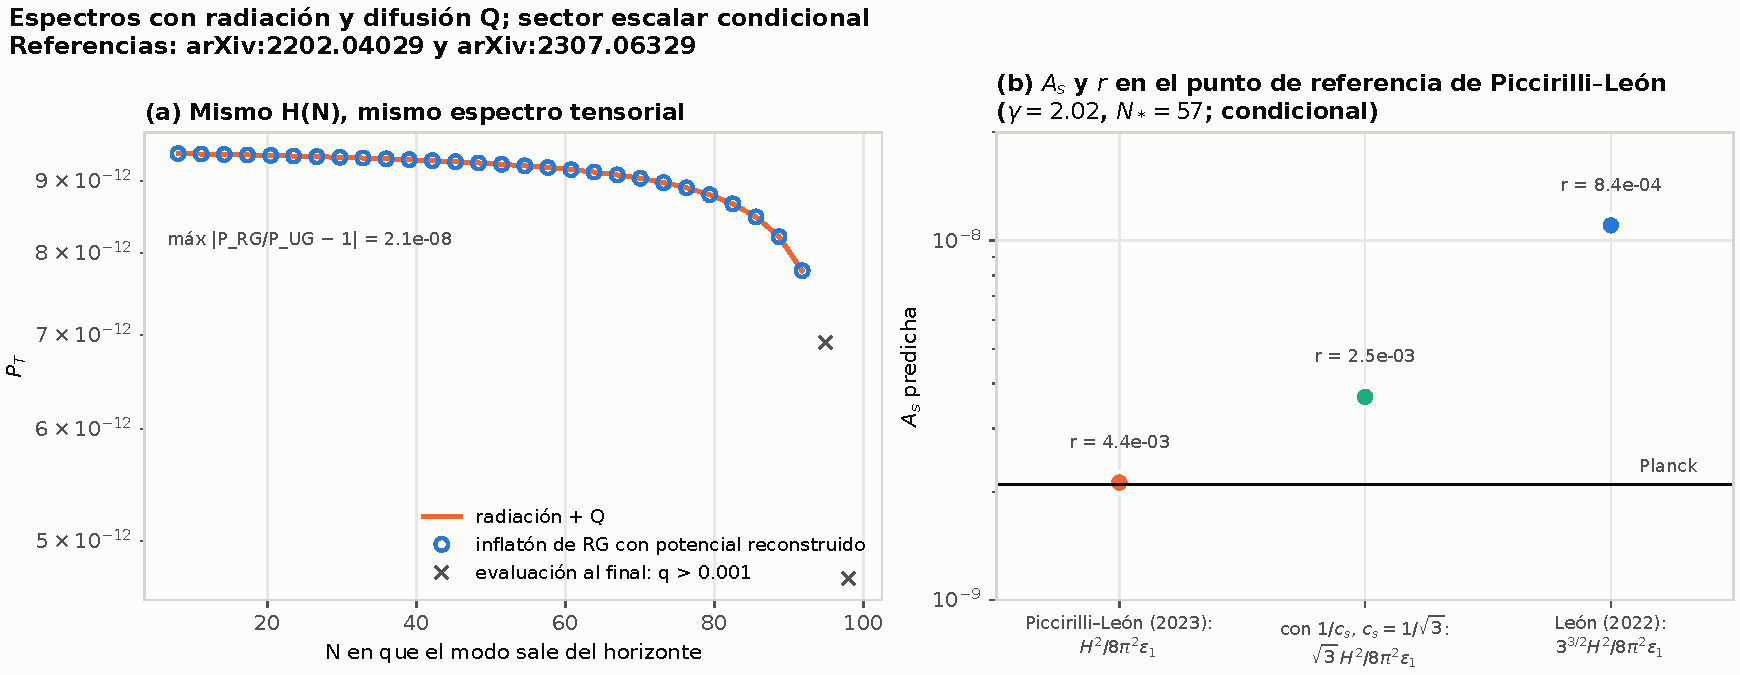
\includegraphics[width=\textwidth]{fig10_leon_PT_As.pdf}
\caption{(a) $P_T$ con radiaci\'on $+Q$ (l\'inea) y con el inflat\'on de RG reconstruido (c\'irculos). (b) $A_s$ y $r$ en el punto de referencia seg\'un tres f\'ormulas escalares (condicional).}
\label{fig:fig10}
\end{figure}

\section{Controles y procedencia}
La validación combina soluciones analíticas de referencia, integración independiente y variaciones de resolución. La malla a igual $k$ permite adelantar el inicio desde $q=k/(aH)=100$ hasta $1000$ y retrasar la evaluación desde $q=10^{-3}$ hasta $10^{-4}$ sin salir del intervalo del fondo. La tabla~\ref{tab:precision} resume la precisión observada en los controles de resolución; sus máximos corresponden a las muestras indicadas, no a una cota global de todos los cálculos.

\begin{table}[htbp]\centering\small
\begin{tabular}{@{}p{0.32\textwidth}p{0.23\textwidth}p{0.37\textwidth}@{}}
\toprule
Control & Máximo observado & Alcance \\
\midrule
Resolución, inicio y parada de los modos & $|\Delta P_T/P_T|=1.03\times10^{-6}$ & Ocho extremos: dos potenciales, RG y UG, dos bordes de la malla. \\
Integrador en tiempo cósmico & $|\Delta P_T/P_T|<4.6\times10^{-10}$ & Los mismos ocho extremos. \\
Paso para calcular $n_T$ & $|\Delta n_T|=6.74\times10^{-7}$ & Ocho índices a $N_*=50,60$; pasos $\Delta\ln k=0.5,0.25,0.125$. \\
\bottomrule
\end{tabular}
\caption{Controles numéricos de los modelos con inflatón. Los criterios exploratorios son $10^{-5}$ para el cambio relativo de potencia y $2\times10^{-5}$ para el cambio absoluto de índice. Este estudio no cubre toda la tabla de radiación con difusión.}
\label{tab:precision}
\end{table}

Además se comprueban el límite exacto de de Sitter (error relativo menor que $10^{-5}$), la expansión slow-roll a segundo orden de \cite{martin14} y el límite conservativo de UG ($\gamma=0$), que recupera RG con diferencias del orden de $10^{-13}$. Se verifica la atribución de las diferencias al fondo, se incluyen controles negativos y mutaciones de código, y se realizan cuatro comprobaciones simbólicas a primer orden y siete controles del modelo de radiación con difusión. Las mutaciones prueban la capacidad de los controles para detectar los errores introducidos; no se conservan pruebas de mutación simbólica.

El registro \texttt{provenance/} reúne entradas, referencias, tablas y datasets de figuras. Su validador comprueba estructura y existencia de archivos y funciones; la prueba de regeneración comprueba sincronía con resultados guardados. Estas verificaciones no certifican por sí solas la verdad científica de las afirmaciones ni ejecutan de nuevo todos los cálculos. La suite de \texttt{make test} contiene 47 pruebas. Los identificadores, los ajustes posteriores de criterio y la ubicación de las salidas se detallan en el apéndice~\ref{app:validacion}.

\section{Discusi\'on y l\'imites}
(i) El resultado tensorial supone materia sin parte TT y la acci\'on tensorial est\'andar como hip\'otesis de la realizaci\'on efectiva; la acci\'on a segundo orden y la equivalencia perturbativa UG$=$RG con $V_{\rm eff}$ no est\'an verificadas simb\'olicamente (una demostraci\'on manual completa alcanzar\'ia; el l\'imite es el alcance). (ii) $Q(N)$ es fenomenol\'ogica; el signo de UG--RG con inflat\'on depende de $\Lambda_0=-Q_i$, del potencial y del criterio. (iii) El argumento sobre $\delta Q=0$ vale para perturbaciones inhomog\'eneas del inflat\'on en el marco especificado; otros gauges y perturbaciones uniformes no se analizaron. (iv) No hay sector escalar de UG con difusi\'on: $A_s$ y $r$ son condicionales y el factor $3^{3/2}$ (puntos O1/O5 del registro de procedencia) sigue abierto; esto es lo pr\'oximo a resolver en la tesis. (v) No se modela el recalentamiento, as\'i que $N_*$ no es la escala observacional (comparar a $N_*=50,60$ es una convenci\'on ilustrativa). (vi) Del modelo de radiación con difusión Q \cite{leon22,piccirilli23} solo se analiz\'o un valor de $\gamma$ adem\'as de $1.5$ y no se reprodujeron los contornos de Planck+BK15 de \cite{piccirilli23}. \emph{Conclusi\'on}: bajo esas hip\'otesis, a igual fondo la propagaci\'on tensorial no distingue UG de RG; las diferencias de los ejemplos provienen del fondo $H(t)$ y del criterio de comparaci\'on. Medir $P_T$ restringe a $Q$ solo por su efecto sobre el fondo, y cu\'anto restringe depende de decisiones que la teor\'ia no fija. El acoplamiento escalar y las f\'ormulas alternativas de $A_s$ son discusi\'on condicionada.

\appendix
\section{Detalle de validación y trazabilidad}
\label{app:validacion}
Los máximos de la tabla~\ref{tab:precision} se conservan en \texttt{codigo/resultados/resolution\_checks.json}. El control de atribución al fondo es C3.4 en \texttt{checks.py}: el valor citado en la sección~\ref{sec:inflaton} corresponde a su muestra del potencial cuadrático y excluye los puntos que no cumplen su criterio slow-roll. El control del mapeo de potenciales es CL7 en \texttt{checks\_leon.py}; sus amplitudes y razones se conservan en \texttt{codigo/resultados/leon/}. Las tolerancias completas y sus revisiones están en los archivos \texttt{checks*.py} y en el registro de procedencia.

Se declararon cuatro ajustes posteriores a observar fallos: (i) la cota NLO de C1.2 para $\epsilon_2\gg\epsilon_1$; (ii) la evaluación de C3.2 desde $N=1$ en Starobinsky, por el salto inicial de $\epsilon_1$; (iii) la restricción de CL1 a los escenarios 1 y 3, porque el escenario 2 es mal condicionado en doble precisión; y (iv) la sustitución, en CL7, del criterio inicial de discrepancia de amplitud menor que $10\%$, que falló, por un criterio exploratorio de diferencia relativa de la razón entre dos escalas menor que $3\%$. Este último cambio no convierte la discrepancia de amplitud en un acuerdo ni valida toda la forma del espectro. Los extremos de la malla publicada se recortaron respecto de la versión inicial para permitir los controles de inicio y parada de los modos.

\begin{thebibliography}{99}
\small
\bibitem{leon22} G.~León, ``Inflation and the cosmological (not-so) constant in unimodular gravity'', \emph{Class.\ Quantum Grav.} \textbf{39}, 075008 (2022), arXiv:2202.04029.
\bibitem{piccirilli23} M.~P.~Piccirilli y G.~León, ``Reconstruction of inflationary scenarios in non-conservative unimodular gravity'', \emph{Mon.\ Not.\ R.\ Astron.\ Soc.} \textbf{524}, 4024 (2023), arXiv:2307.06329.
\bibitem{bengochea23} G.~R.~Bengochea, G.~León, A.~Perez y D.~Sudarsky, ``A clarification on prevailing misconceptions in unimodular gravity'', \emph{JCAP} \textbf{11} (2023) 011, arXiv:2308.07360.
\bibitem{fabris22} J.~C.~Fabris, M.~H.~Alvarenga, M.~Hamani Daouda y H.~Velten, ``Nonconservative unimodular gravity: gravitational waves'', \emph{Symmetry} \textbf{14}, 87 (2022), arXiv:2112.06663.
\bibitem{martin14} J.~Martin, C.~Ringeval y V.~Vennin, ``Encyclopaedia Inflationaris'', arXiv:1303.3787v3 (se usa la numeración de ecuaciones de la versión v3).
\bibitem{planck20} Planck Collaboration, ``Planck 2018 results. X. Constraints on inflation'', \emph{Astron.\ Astrophys.} \textbf{641}, A10 (2020), arXiv:1807.06211.
\bibitem{bicep21} BICEP/Keck Collaboration, ``Improved constraints on primordial gravitational waves using Planck, WMAP, and BICEP/Keck observations through the 2018 observing season'', \emph{Phys.\ Rev.\ Lett.} \textbf{127}, 151301 (2021), arXiv:2110.00483.
\bibitem{starobinsky80} A.~A.~Starobinsky, ``A new type of isotropic cosmological models without singularity'', \emph{Phys.\ Lett.\ B} \textbf{91}, 99 (1980), DOI 10.1016/0370-2693(80)90670-X.
\bibitem{defelice10} A.~De Felice y S.~Tsujikawa, ``$f(R)$ theories'', \emph{Living Rev.\ Relativ.} \textbf{13}, 3 (2010), arXiv:1002.4928.
\bibitem{garriga99} J.~Garriga y V.~F.~Mukhanov, ``Perturbations in k-inflation'', \emph{Phys.\ Lett.\ B} \textbf{458}, 219 (1999), hep-th/9904176.
\bibitem{baumann22} D.~Baumann, \emph{Cosmology} (Cambridge University Press, 2022); y ``TASI lectures on inflation'', arXiv:0907.5424.
\bibitem{josset17} T.~Josset, A.~Perez y D.~Sudarsky, ``Dark energy from violation of energy conservation'', \emph{Phys.\ Rev.\ Lett.} \textbf{118}, 021102 (2017), arXiv:1604.04183.
\end{thebibliography}
\end{document}
